
\chapter{Literature Review}\label{chap:LR} \markright{\thechapter~Literature Review}
This chapter reviews the current state of research relevant to the sustainability assessment of structural systems, with particular emphasis on floor structures. The review focuses on embodied carbon, material performance, structural efficiency, and the indirect influence of structural system choices on overall building performance. The discussion of material performance identifies timber and concrete floor systems as the most relevant structural solutions within the scope of this thesis. In addition, social and economic aspects relevant to floor systems are examined, including serviceability and comfort requirements, construction productivity, and cost-related considerations. Based on this review, the factors used to assess the sustainability of floor systems in this thesis are identified.

The floor systems considered within the scope of this thesis are presented in the following section. They are compared with respect to their prevalence in practice, material composition, structural efficiency, constructability, economic performance, and functional characteristics to justify their selection for further investigation.


\section{Ecological sustainability of structural systems \label{Sec: SustainabilityAss}}

\subsection{Emissions per unit mass of material}
The most obvious influence on a structure's total environmental impact is the material-specific footprint. If the mechanical properties of a material can be maintained while reducing its embodied carbon intensity ($kgCO_2/kg$), the overall environmental footprint can be reduced.
For instance, as concrete is by far the most widely used building material globally, efforts to reduce carbon-intensive clinker by incorporating supplementary cementitious materials have represented one of the primary levers for decarbonisation for several decades \cite{artDigConc, Snellings2023}. Current research continues to expand this scope, focusing on the development of alternative low-carbon binders and the implementation of carbon capture, utilisation, and storage technologies \cite{Barbhuiya2024}. Across all material groups, such advancements have resulted in a complex and diverse landscape of materials with unique environmental profiles that must be carefully accounted for in any structural sustainability assessment.

To evaluate the environmental values of construction materials, Environmental Product Declarations (EPDs) serve as the primary quantitative source. These documents provide a standardised framework for assessing manufacturer-specific ecological impacts, such as the Global Warming Potential (GWP), in accordance with ISO 14025 \cite{ISO_14025} and EN 15804 \cite{EN_15804}. As EPDs are manufacturer-specific, they enable accurate comparisons that account for the variance within a single material group (e.g. concrete of strength class C30/37 or structural timber of grade C24). These variations become particularly significant when considering that the specific supplier or manufacturer of a building material is often determined only in the later design stages of a project \cite{Kaufmann2024_WhitePaper}. It can be concluded that a comprehensive environmental sustainability analysis must take these variations into account.


\subsection{Material performance per mass of material} 
\subsubsection{Material performance}
The emissions of a construction material should always be rated based on the mechanical performance achieved per unit of emission, particularly its strength, stiffness and ductility \cite{Kaufmann2024_WhitePaper}. To evaluate the material performance, a load-deformation diagram \ref{fig:LDdiagrams} can be used. The results indicate that the ranges of load-deformation behaviour overlap notably across different materials due to the variation in embodied carbon values of the EPDs. Still, timber and reinforced concrete show the highest stiffness and strength under compression. For tension members, timber and prestressed concrete show the best stiffness. As stiffness often becomes the governing factor for slab structures due to rigorous deformation limits, concrete and timber systems therefore become particularly relevant.


\begin{figure}[H]
    \centering
    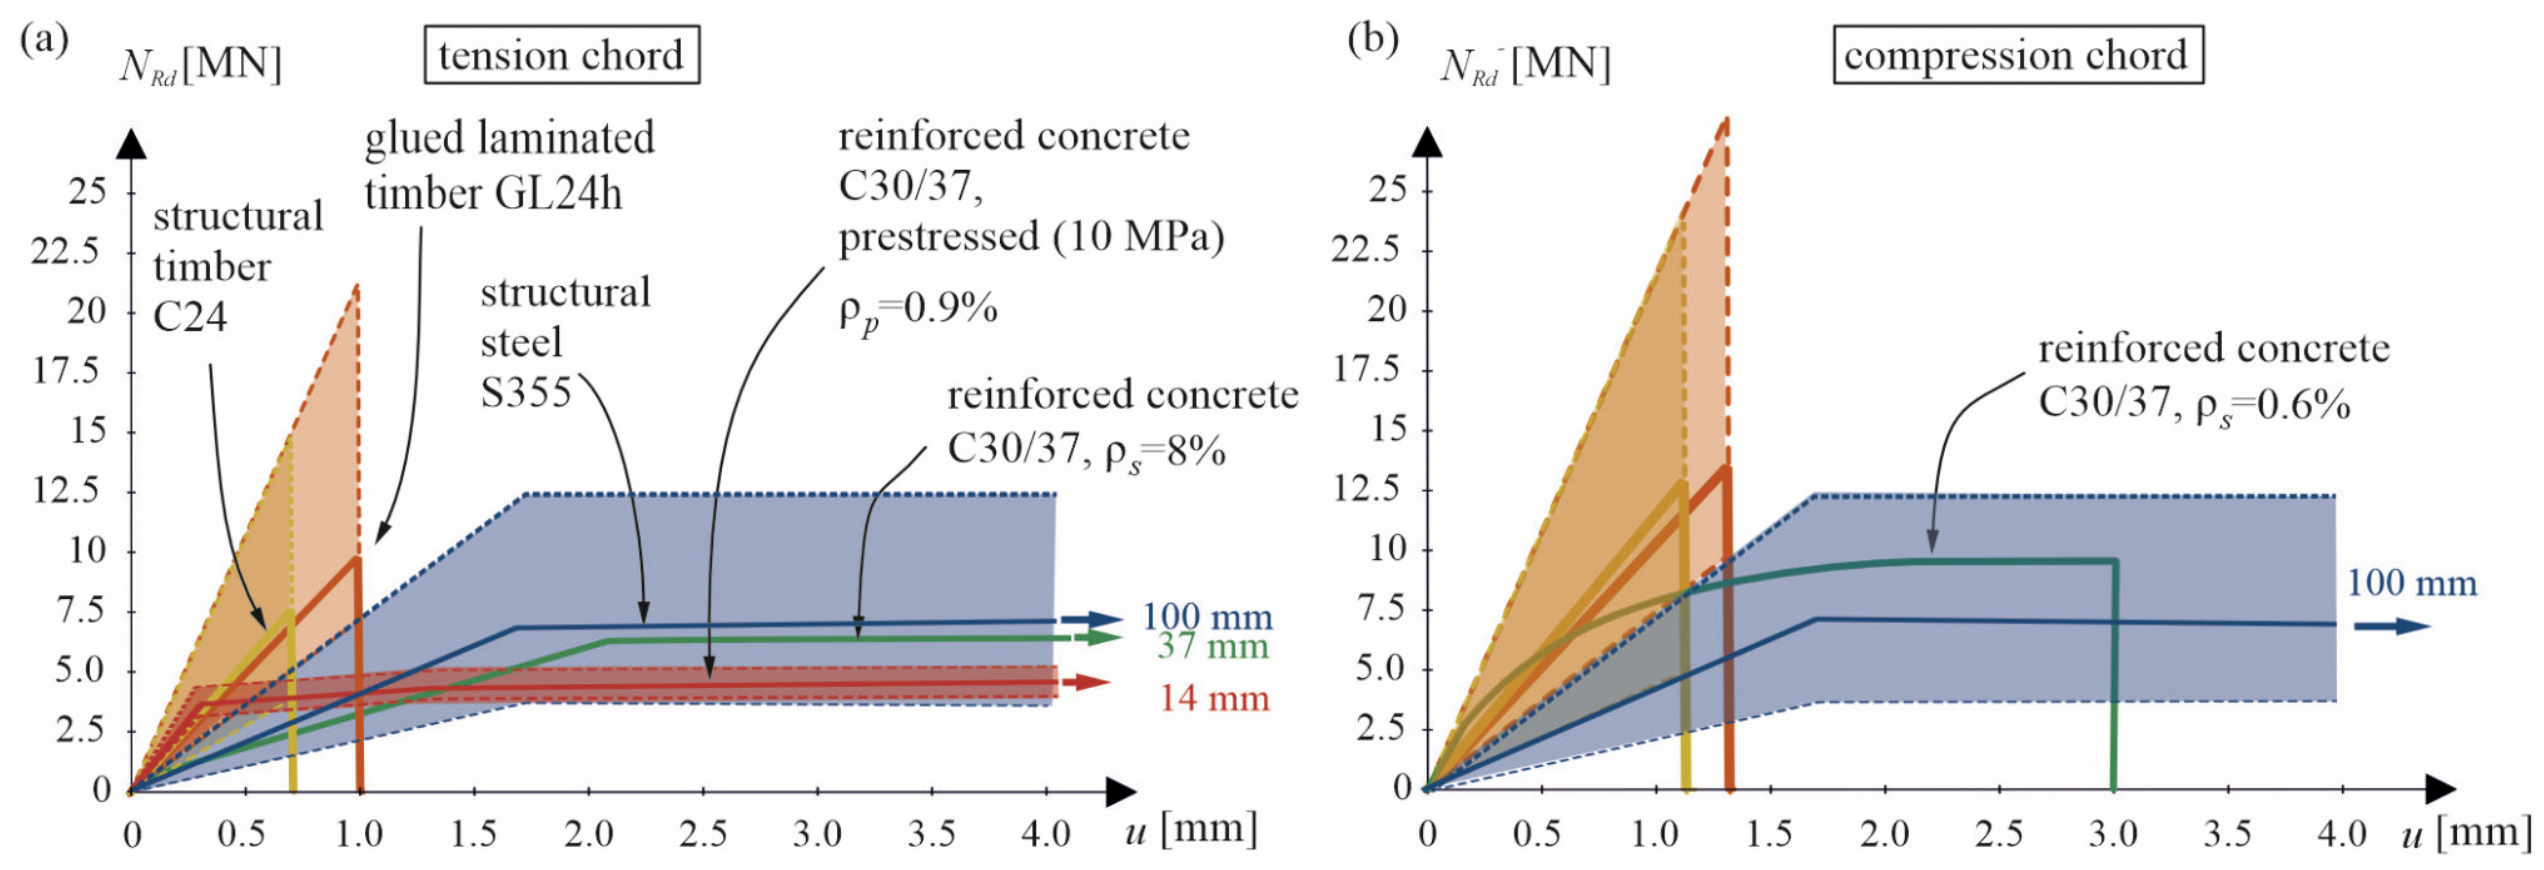
\includegraphics[width=0.9\textwidth]{IMAGES/LoadDeformationDiagram.png}
    \caption{Load-deformation diagrams of (a) tension and (b) compression members using structural timber, steel and reinforced (prestressed) concrete with a consumption of $100\ kg CO_{2}eq$ per running metre \cite{kfmResearch2026}.}
    \label{fig:LDdiagrams}
\end{figure}

A material with a higher initial embodied carbon per kilogram may prove more ecologically efficient if its superior mechanical capacity permits a significant reduction in the total volume of material required for the structure. However, this efficiency heavily depends on what becomes the governing design criterion. For example, the use of high-strength concrete has a considerably greater impact on strength than on stiffness, meaning the ecological benefit varies depending on the governing limit state.  Thus, over-designed elements must be avoided to ensure that the inherent mechanical capacity of the material is fully utilised.

\subsubsection{Efficiency of cross section}
The structural efficiency of a member is defined not only by the material used, but also by the geometric distribution of its cross section. Placing the same amount of material further away from the neutral axis increases the bending stiffness quadratically, according to Steiner’s theorem. Unfortunately, for slab structures, a flat ceiling is often desired to accommodate building services and to minimise overall storey height. Furthermore, complex cross sections are frequently more expensive to construct. In the past, material-efficient geometries, such as ribbed slabs, were the standard because material costs were relatively high compared to labour costs. This economic dynamic has since inverted, promoting the use of simpler but more material-intensive cross sections, such as solid rectangular concrete profiles \cite{Kaufmann2024_WhitePaper}.

\subsubsection{Efficiency of structural system}
The structural efficiency of a slab system is mainly influenced by the span of the system, whether it spans in one or multiple directions, and the continuity over the support. To illustrate this: A two-way spanning slab with continuity exhibits only one-tenth of the deflections compared to a one-way simply supported system, enabling much slender cross-sections. Whether continuity is achievable depends heavily on the chosen materialisation, as further elaborated in Section \ref{Sec: FloorSyst}. Furthermore, the span length largely influences the governing design criteria, with internal bending moments scaling proportionally to the span squared and deflections scaling proportionally to the span to the fourth power. Consequently, designers must strike a careful balance between selecting shorter spans to maximise structural and material efficiency, and maintaining adequate spatial flexibility to ensure a long service life for the building \cite{Kaufmann2024_WhitePaper}.


\subsection{Indirect influences \label{Sec: IndirectInfl}}

The loading of a structure is governed by its use. However, designers should critically review and discuss the loading scenario. For example, heavy and thick earth cover or unnecessarily high live load assumptions should be avoided. Often, structures are designed for heavier load scenarios for flexibility in the future. Similarly, non-continous systems are used for easier deconstruction for circularity purposes.
Those upfront carbon investments should always be taken with caution and only where a different scenario of use is intended, as designing a more efficient structure tailored for current needs will yield a lower overall environmental footprint \cite{Kaufmann2024_WhitePaper}.

The design choices of the structural system also have indirect influences on the overall environmental performance of the building in consequence. First, the total height of the structure plays a critical role. Increasing the depth of the member directly increases the total facade area and insulation area and reduces the usable floor space within a given zoning envelope. Second, the total mass of the building governs the design of the foundation, as higher structural loads require more foundation material. Both factors also increase the horizontal load through wind and earthquake, resulting in more extensive lateral load-resisting systems \cite{Kaufmann2024_WhitePaper}.

\section{Social and economic considerations}
Sustainability is generally defined in terms of its ecological, social, and economic dimensions \cite{Ammann2024}. Thus, the ecological sustainability assessment of Section \ref{Sec: SustainabilityAss} must be extended to satisfy user comfort, construction cost, and productivity requirements. Beyond these aspects, there are further considerations, such as health-related aspects. However, these are assumed to be outside the scope of this thesis.

\subsection{Serviceability and comfort \label{Sec: ServAndComf}}
In addition to limiting deflections, floor systems must satisfy vibration requirements to ensure adequate user comfort. This aspect becomes particularly relevant for lightweight floor systems due to their comparatively low stiffness and mass. Furthermore, floor systems must fulfil acoustic requirements, including both airborne and impact sound insulation. Achieving sufficient acoustic performance may require additional floor build-ups or increased structural mass. Consequently, lightweight floor systems often require additional measures to satisfy vibration and acoustic requirements, partially offsetting their ecological advantages \cite{BauphysikKalender}.

Particularly in Switzerland, these requirements are stringent and the expected level of comfort is high. Reducing these limits with respect to ecological sustainability is possible, but requires the client's approval \cite{Kaufmann2024_WhitePaper}. As these limits are very important for general health and public well-being, they should not be treated as soft constraints from the outset. However, assessing which criteria govern a specific floor system can help identify whether a discussion regarding comfort requirements in relation to ecological sustainability may be necessary.

\subsection{Importance of construction cost \label{Sec: ConstructionCost}}
The construction sector is a cost-driven environment, as competitive bidding is standard practice. Economically uncompetitive solutions will not to lead to widespread use. Therefore, for a practice-oriented comparison, the costs should also be taken into account to ensure financially feasible designs.

In advanced economies, labour cost is the most significant cost driver. Consequently, structurally or environmentally optimised systems are often not economically competitive. Ammann et al. \cite{Ammann2024} therefore state that “a conflict often arises between GWP and cost” when selecting a structural system. For this reason, the cost of a floor system is considered an important factor in the sustainability assessment.

\subsection{Construction productivity \label{Sec: Productivity}}
Compared to other industrial sectors, the construction industry has experienced only limited productivity improvements in recent decades \cite{Wangler2019}. As a result, improving construction productivity represents an important aspect of the future development of the construction industry.

In this context, prefabrication in combination with Building Information Modelling (BIM) offers significant potential to improve efficiency and reduce labour demand on-site \cite{Caulfield2022}. Furthermore, systems that enable faster construction progress, such as prefabricated timber elements or post-tensioned slabs with reduced propping times \cite{Rombach2010}, may help compensate for higher production costs or more complex geometries.

\section{Key factors that define sustainability}
The factors identified in the literature review serve as comparison criteria for evaluating the sustainability performance of floor systems. Sustainability is understood as comprising environmental, social, and economic dimensions. The assessment is carried out both for the structural slab alone and for the complete floor system, which includes the floor build-up required to meet acoustic insulation requirements.

\newcolumntype{L}[1]{>{\raggedright\arraybackslash}p{#1}}

\begin{table*}[h]
    \centering
    \begingroup
    \scriptsize
    \setlength{\tabcolsep}{4pt}
    \renewcommand{\arraystretch}{1.2}
    \begin{tabularx}{\textwidth}{@{}L{2.8cm}|L{3.6cm}|L{1.6cm}|X@{}}
    \hline
    \textbf{Name} &
    \textbf{Parameter} &
    \textbf{Unit} &
    \textbf{Reason} \\ \hline

    Global Warming Potential &
    $GWP_{\mathrm{struct}}$, $GWP_{\mathrm{tot}}$ &
    kg CO$_2$-eq/m$^2$ &
    Section \ref{Sec: SustainabilityAss}: GWP of the cross-section for its specific structural system while accounting for producer-specific material variations.  \\

    Height &
    $h_{\mathrm{struct}}$, $h_{\mathrm{tot}}$ &
    m &
    Section \ref{Sec: IndirectInfl}: Indirect influence total height.  \\

    Mass &
    $m_{\mathrm{struct}}$, $m_{\mathrm{tot}}$ &
    kN/m$^2$ &
    Section \ref{Sec: IndirectInfl}: Indirect influence total mass.  \\

    Cost &
    $cost_{\mathrm{struct}}$, $cost_{\mathrm{tot}}$ &
    CHF/m$^2$ &
    Section \ref{Sec: ConstructionCost}: Economic sustainability and market competitiveness\\

    Construction time &
    $T_{\mathrm{struct}}$, $T_{\mathrm{tot}}$ &
    h/m$^2$ &
    Section \ref{Sec: Productivity}: Productivity  \\ \hline
    \end{tabularx}
    \endgroup
    \caption{Sustainability factors for slab comparison. \label{Tab: SustFact}}
\end{table*}

\begin{table*}[h]
    \centering
    \begingroup
    \scriptsize
    \setlength{\tabcolsep}{4pt}
    \renewcommand{\arraystretch}{1.2}
    \begin{tabularx}{\textwidth}{@{}L{2.8cm}|L{5.0cm}|X@{}}
    \hline
    \textbf{Requirement} &
    \textbf{Limit} &
    \textbf{Verification in the slab configurator} \\ \hline

    ULS &
    $q_{k,\mathrm{zul,GZT}} \geq q_k$ &
    Ultimate limit state verification of bending and shear resistance under design load combinations \cite{SIA260_2013, SIA261_2020}. \\

    SLS 1 &
    $w_{\mathrm{install}} \leq L/350$
    
    $w_{\mathrm{use}} \leq L/350$
    
    $w_{\mathrm{app}} \leq L/300$ &
    Serviceability limit state verification of deflections, including installation, use and appearance deflection limits \cite{SIA260_2013, SIA261_2020}. \\

    SLS 2 &
    $f_1 \geq f_{1,\min}$, $a_{\mathrm{ed}} \leq a_{\mathrm{lim}}$, $w_{f,\mathrm{ed}} \leq w_{f,\mathrm{lim}}$, $v_{\mathrm{ed}} \leq v_{\mathrm{cd}}$ &
    Serviceability limit state verification of vibration behaviour, including natural frequency and vibration response checks \cite{Lignum3.1:2015, Ziegler2008Grundlagen}. \\

    Fire &
    $R_{\mathrm{fire}} \geq 60\,\mathrm{min}$ &
    Fire resistance verification according to the section-specific fire exposure and material rules \cite{SIA260_2013}. \\

        Acoustic requirements &
    Normal (Increased): $R_w \geq 53\,(57)\,\mathrm{dB}+\Delta_{\mathrm{plan}}$
    $L_{n,w} \leq 51\,(47)\,\mathrm{dB}-\Delta_{\mathrm{plan}}$
    
    $\Delta_{\mathrm{plan}}=5\,\mathrm{dB}$ for concrete
    $\Delta_{\mathrm{plan}}=8\,\mathrm{dB}$ for timber &
    Automated generation of the floor build-up to fulfil the selected acoustic requirement level, including airborne and impact sound checks \cite{SIA181_2020}. \\ \hline
    \end{tabularx}
    \endgroup
    \caption{Requirements according to the Swiss national standard that are fulfilled by the slab configurator.}
    \label{tab:configurator_requirements}
    \label{Tab: ReqSS}
\end{table*}

\section{Major types of floor systems\label{Sec: FloorSyst}}
For the purposes of this comparison, the floor systems most commonly used in building construction are identified and supplemented by more advanced alternatives that promise improved sustainability performance. Residential and office buildings represent the application area. Although the floor systems considered are used internationally, the review is tailored to the Swiss construction market. Furthermore, economic considerations, such as the comparatively high labour costs, are based on Swiss market conditions. In doing so, this section focuses on the broader system level. More refined modelling assumptions and considerations are introduced in Chapter \ref{sec:MM}.

Steel-concrete composite floor systems are not considered in this study, as they have historically seen limited application in Switzerland \cite{Mensinger2010}. Furthermore, digitally fabricated slabs and highly structurally optimised solutions are excluded, as they are not yet considered ready for widespread adoption in building practice and remain insufficiently covered by current design standards and regulations \cite{Wangler2019, Ranaudo2021HiLo}.



\subsection{Solid reinforced concrete slab}
The solid reinforced concrete slab is the current industry standard in Switzerland \cite{Ammann2024}. Local construction companies possess the necessary formwork systems, supports and the expertise gained through decades of practice, making this system economically competitive. Due to its geometric simplicity, flexibility for building service installations, inherent fire resistance and acoustic insulation, planners typically favour this system. Structurally, it relies on an efficient two-way load-bearing mechanism with continuity over the supports. However, in terms of cross-sectional performance, the flat slab is inefficient from a sustainability perspective. A significant portion of the concrete in the tension zone does not contribute to the structural capacity but adds considerable self-weight and embodied carbon.

\subsection{Ribbed reinforced concrete slab}
Ribbed slabs optimise material usage by concentrating concrete in the compression zone and utilising ribs in the tension zone to house the reinforcement. As a result, the self-weight is reduced, allowing for longer spans. However, the improved structural efficiency leads to an increased construction height and potentially reduced functionality of the floor system. The more refined cross-section requires complex formwork and a higher amount of manual labour, increasing costs especially in countries with high labour costs \cite{Ammann2024, Kaufmann2024_WhitePaper}.

\subsection{Post-tensioned solid concrete slab}
Looking at the current market situation, there is no denying that the advantages of a solid slab are important. Reduced overall height, spatial flexibility, unobstructed installation of building services, combined with the lowest cost per square metre of slab \cite{Ammann2024}. Thus, post-tensioned solid concrete slabs with unbonded tendons were included in the investigation as a system that combines the advantages of an inefficient solid slab with the structural efficiency provided by prestressing. \cite{Rombach2010}

Post-tensioned slabs introduce active compressive stresses into the concrete through high-strength steel tendons. As a result, post-tensioned slabs stay longer in the uncracked state, showing higher bending stiffnesses. Depending on the tendon trajectory, deviation forces can compensate part of the applied load. The degree of post-tensioning determines the extent to which the loads are balanced. \cite{Rombach2010, flachdecken_Morgen} 
Both effects improve serviceability behaviour with respect to deflections and enable longer spans or reduced slab thicknesses compared with conventional reinforced concrete slabs. Consequently, in the context of sustainability-optimised floor systems, post-tensioned slabs represent a major competitor, as they can reduce the required quantities of concrete and reinforcing steel while simultaneously minimising the overall building height.

For point supports, the punching behaviour is improved. The applied action is reduced by tendon deviation forces, while the resistance is increased through reduced slab rotations.

Post-tensioning solid slabs through unbonded tendons is not a new system. Early tendon layouts for two-way post-tensioned slabs, developed in the 1950s in the United States, typically consisted of uniformly distributed tendons with additional tendons in the support strips \cite{PTI2023}. However, these layouts increased the complexity of future slab penetrations \cite{Rombach2010}. Dual-banded layouts address this limitation and further improve the existing system. Here, the tendons are concentrated within the support strips above the columns. Advantageously, dual-banded prestressing leaves the central regions of the slab largely free of tendons, allowing penetrations and openings to be added with minimal risk of damaging tendons. In addition, the concentration of tendons along the column strips simplifies tendon installation, reduces coordination conflicts with other building services, and improves the practicality of slab optimisations in the span region, such as voided or waffle slab constructions \cite{PTI2023}.

\begin{figure}[htbp]
    \centering
    \resizebox{\textwidth}{!}{%
        \definecolor{tendonblue}{HTML}{1F4E99}

\begin{tikzpicture}[
    slab/.style={black, thick},
    tendon/.style={tendonblue, thin},
    gridline/.style={gray!45, dashed, thin},
    support/.style={draw, fill=gray!30, minimum size=0.28cm, inner sep=0pt},
    dim/.style={<->, thin},
    tick/.style={thin},
    txt/.style={font=\scriptsize},
    subtit/.style={font=\scriptsize\bfseries},
    note/.style={font=\scriptsize, align=center}
]

% Dimensions
\def\W{6.0}
\def\H{6.0}
\def\bayX{2.0}
\def\bayY{2.0}
\def\xA{0}
\def\xB{8.0}
\def\y{0}

% ============================================================
% (a) Distributed layout
% ============================================================

% Slab outline
\draw[slab] (\xA,\y) rectangle ++(\W,\H);

% Column grid lines
\foreach \xx in {0,2,4,6} {
    \draw[gridline] (\xA+\xx,\y-0.15) -- (\xA+\xx,\y+\H+0.15);
}
\foreach \yy in {0,2,4,6} {
    \draw[gridline] (\xA-0.15,\y+\yy) -- (\xA+\W+0.15,\y+\yy);
}

% Supports
\foreach \xx in {0,2,4,6} {
    \foreach \yy in {0,2,4,6} {
        \node[support] at (\xA+\xx,\y+\yy) {};
    }
}

% Distributed tendons aligned with column grid and extending to slab edges
\foreach \xx in {0,0.5,1.0,1.5,2.0,2.5,3.0,3.5,4.0,4.5,5.0,5.5,6.0} {
    \draw[tendon] (\xA+\xx,\y) -- (\xA+\xx,\y+\H);
}
\foreach \yy in {0,0.5,1.0,1.5,2.0,2.5,3.0,3.5,4.0,4.5,5.0,5.5,6.0} {
    \draw[tendon] (\xA,\y+\yy) -- (\xA+\W,\y+\yy);
}

% Dimensions x
\foreach \xx in {0,2,4} {
    \draw[dim] (\xA+\xx,\y+\H+0.45) -- (\xA+\xx+2,\y+\H+0.45);
    \draw[tick] (\xA+\xx,\y+\H+0.30) -- (\xA+\xx,\y+\H+0.60);
    \draw[tick] (\xA+\xx+2,\y+\H+0.30) -- (\xA+\xx+2,\y+\H+0.60);
    \node[txt] at (\xA+\xx+1,\y+\H+0.72) {$l_x$};
}

% Dimensions y
\foreach \yy in {0,2,4} {
    \draw[dim] (\xA+\W+0.45,\y+\yy) -- (\xA+\W+0.45,\y+\yy+2);
    \draw[tick] (\xA+\W+0.30,\y+\yy) -- (\xA+\W+0.60,\y+\yy);
    \draw[tick] (\xA+\W+0.30,\y+\yy+2) -- (\xA+\W+0.60,\y+\yy+2);
    \node[txt] at (\xA+\W+0.75,\y+\yy+1) {$l_y$};
}

% ============================================================
% (b) Banded layout
% ============================================================

% Slab outline
\draw[slab] (\xB,\y) rectangle ++(\W,\H);

% Column grid lines
\foreach \xx in {0,2,4,6} {
    \draw[gridline] (\xB+\xx,\y-0.15) -- (\xB+\xx,\y+\H+0.15);
}
\foreach \yy in {0,2,4,6} {
    \draw[gridline] (\xB-0.15,\y+\yy) -- (\xB+\W+0.15,\y+\yy);
}

% Supports
\foreach \xx in {0,2,4,6} {
    \foreach \yy in {0,2,4,6} {
        \node[support] at (\xB+\xx,\y+\yy) {};
    }
}

% Banded tendons along column strips, extending to slab edges
\foreach \yy in {0,2,4,6} {
    \foreach \dy in {-0.18,-0.09,0,0.09,0.18} {
        \draw[tendon] (\xB,\y+\yy+\dy) -- (\xB+\W,\y+\yy+\dy);
    }
}

\foreach \xx in {0,2,4,6} {
    \foreach \dx in {-0.18,-0.09,0,0.09,0.18} {
        \draw[tendon] (\xB+\xx+\dx,\y) -- (\xB+\xx+\dx,\y+\H);
    }
}

% Dimensions x with xi notation
\draw[dim] (\xB,\y+\H+0.45) -- (\xB+2,\y+\H+0.45);
\node[txt] at (\xB+1,\y+\H+0.72) {$l_x$};

\draw[dim] (\xB+2,\y+\H+0.45) -- (\xB+2.35,\y+\H+0.45);
\node[txt] at (\xB+2.175,\y+\H+0.72) {$\xi l_x$};

\draw[dim] (\xB+2.35,\y+\H+0.45) -- (\xB+3.65,\y+\H+0.45);
\node[txt] at (\xB+3.0,\y+\H+0.72) {$(1-2\xi)l_x$};

\draw[dim] (\xB+3.65,\y+\H+0.45) -- (\xB+4.0,\y+\H+0.45);
\node[txt] at (\xB+3.825,\y+\H+0.72) {$\xi l_x$};

\draw[dim] (\xB+4,\y+\H+0.45) -- (\xB+6,\y+\H+0.45);
\node[txt] at (\xB+5,\y+\H+0.72) {$l_x$};

\foreach \xx in {0,2,2.35,3.65,4,6} {
    \draw[tick] (\xB+\xx,\y+\H+0.30) -- (\xB+\xx,\y+\H+0.60);
}

% Dimensions y
\foreach \yy in {0,2,4} {
    \draw[dim] (\xB+\W+0.45,\y+\yy) -- (\xB+\W+0.45,\y+\yy+2);
    \draw[tick] (\xB+\W+0.30,\y+\yy) -- (\xB+\W+0.60,\y+\yy);
    \draw[tick] (\xB+\W+0.30,\y+\yy+2) -- (\xB+\W+0.60,\y+\yy+2);
    \node[txt] at (\xB+\W+0.75,\y+\yy+1) {$l_y$};
}

% Installation / optimisation field
\fill[magenta!25, draw=magenta!25, solid, thick]
    (\xB+4.2,\y+0.2) rectangle ++(1.6,1.6);
\node[note, magenta!90!black, font=\tiny] at (\xB+5,\y+0.70)
    {Installation /\\Optimisation};
\end{tikzpicture}%
}
    }
    \caption{Comparison of (a) distributed and (b) banded layouts for two-way post-tensioned slabs.}
    \label{fig:distributed_banded_tendon_layouts}
\end{figure}


\subsection{Solid timber slab}
Timber as a material offers a higher strength-to-weight ratio with a lower environmental impact than steel, making it an attractive structural material \cite{Wimmers2017}. Solid timber systems, primarily utilising glulam or cross-laminated timber elements, offer a high degree of prefabrication.
Due to the modular nature of timber construction, achieving continuity over supports is often challenging, resulting in the widespread use of simply supported systems. Furthermore, timber structures are generally designed elastically, as the brittle tensile failure of wood limits the potential for plastic redistribution. In contrast, reinforced concrete and steel structures are better suited for the development of hyperstatic continuous structural systems, in which internal force redistribution allows for increased bearing capacity.

Although wood is a combustible material, its fire behaviour can be predicted reliably, making its application feasible provided that a rigorous fire design is implemented \cite{frangi2008fire}. However, due to the comparatively low stiffness and mass of timber structures, timber slabs are frequently governed by serviceability limit states, particularly vibration and deflection criteria, rather than ultimate strength. In addition, the low mass of timber results in comparatively poor acoustic insulation, often requiring heavy and costly floor build-ups to meet regulatory requirements \cite{Kaufmann2024_WhitePaper}.


\subsection{Ribbed and hollow-core timber slabs}
These systems, such as timber ribs with a top (and bottom) plate, aim to increase the moment of inertia while maintaining the lightweight benefits of wood. Hollow cores are often used for acoustic insulation or integration of building services \cite{Frangi2009_HC}. Compared to mass timber, hollow-core systems are more complex to fabricate and often incorporate a variety of different materials, which can negatively affect their circularity and ease of deconstruction. However, hollow-core systems are typically delivered as prefabricated elements, enabling rapid construction progress on-site.

\subsection{Timber-concrete composite slabs}
These composite slabs combine the strengths of two distinct materials. Concrete is placed in the upper compression zone to provide stiffness, fire protection, and acoustic mass, while timber is used in the lower tension zone. Consequently, less reinforcement and concrete are required compared to a conventional reinforced concrete system, while acoustic insulation and fire protection are ensured by the concrete topping \cite{proHolz2012_Zuschnitt45}. The degree of composite action is governed by the stiffness of the shear connection between the two materials \cite{Eurocode5_2023}.

As with pure timber systems, timber-concrete composite systems lack complete continuity over the supports. Promisingly, there is sustained effort to enable at least partial continuity in the case of in-situ concrete \cite{durchlauf_HBV}. This is addressed in upcoming standards through the calculation of a single-span system with a reduced effective span \cite{Eurocode5_2023}.

\subsubsection{Solid timber-concrete composite slabs}
A solid timber-concrete composite slab typically consists of a glulam, cross-laminated timber or solid timber deck with a concrete topping. This configuration is frequently used in residential buildings, as structural and acoustic requirements can be met while maintaining a relatively slim profile. In such cases, notches in the timber panel are typically used as shear connectors \cite{proHolz2012_Zuschnitt45, Eurocode5_2023}.

\subsubsection{Ribbed timber-concrete composite slabs}
The ribbed timber-concrete composite slab uses solid timber- or glulam beams acting compositely with a thin concrete flange. This material-efficient composite system is capable of achieving longer spans with a very low self-weight-to-stiffness ratio. Here, screws, bonded steel rods, or steel plates are typically used as shear connectors \cite{proHolz2012_Zuschnitt45}.


\section{Quantify sustainability}
The three commonly acknowledged dimensions of sustainability are environmental, social and
economic sustainability \cite{Ammann2024}
